%\documentclass{clases}
\documentclass[a4paper,12pt, oneside]{book}
\usepackage[skins,minted]{tcolorbox}
\usepackage[utf8]{inputenc}
\usepackage[T1]{fontenc}
\usepackage[spanish, es-tabla]{babel}
\languageshorthands{spanish}
%\usepackage{lmodern} % Usa las fuentes modernas de LaTeX
\usepackage[numbers]{natbib}
%\usepackage{morewrites}
\usepackage{inconsolata}
\usepackage{mdframed}
\usepackage{minted}
\usepackage{bm}
\usepackage{listingsutf8}
\usepackage{subcaption}
\usepackage{amsmath}
\usepackage{amssymb}
\usepackage{graphicx}
\usepackage{hyperref}
\usepackage{longtable}
\usepackage{tabularx}
\usepackage{threeparttable}
\usepackage{array}    % Necesario para centrar horizontal y verticalmente
\usepackage{xcolor}
\usepackage{pdfpages}
%\usepackage{color}
\usepackage{fancyhdr}
\usepackage{menukeys}
\usepackage{appendix}
\usepackage{fontawesome}
\usepackage{comment}
\usepackage{caption}
\usepackage{setspace}
\usepackage[explicit]{titlesec}
\usepackage[a4paper,margin=2cm]{geometry}

%\geometry{top=3cm, bottom=3cm, left=4cm, right=2cm} % Si lo quieres imprimir

\definecolor{green1}{HTML}{1dae28}
\definecolor{green2}{HTML}{afd095}
\definecolor{lightgray}{gray}{0.9}
\definecolor{orange}{RGB}{18,84,183}
\definecolor{titulo}{gray}{0.75}
\definecolor{gray97}{gray}{.97}
\definecolor{gray75}{gray}{.75}
\definecolor{gray45}{gray}{.45}
\definecolor{advertencia}{RGB}{255,178,102}
\definecolor{colorturqueza}{RGB}{178,223,238}
\definecolor{mintedbackground}{rgb}{0.95,0.95,0.95}
\definecolor{lbcolor}{rgb}{0.95,0.95,0.95}
\definecolor{mintedframe}{rgb}{0.0,0.0,0.0}
\definecolor{codebg}{rgb}{0.96,0.96,0.96}
\definecolor{colorurls}{RGB}{107,17,17}
\definecolor{colorsql}{RGB}{255,245,245}
\definecolor{colorreferences}{RGB}{48,134,3}
\definecolor{titulo}{gray}{0.65}			%------ color para fondo del titulo de tablas.

\hypersetup{
	%bookmarks=true,         % show bookmarks bar?
	unicode=true,          % non-Latin characters in Acrobat’s bookmarks
	pdftoolbar=true,        % show Acrobat’s toolbar?
	pdfmenubar=true,        % show Acrobat’s menu?
	pdffitwindow=false,     % window fit to page when opened
	pdfstartview={FitH},    % fits the width of the page to the window
	pdftitle={Reporte final de Robótica},    % title
	%	pdfauthor={},     % author
	pdfsubject={Reporte final de Robótica},   % subject of the document
	%pdfcreator={pdfTeX 3.14159265-2.6-1.40.16 (TeX Live 2016/dev)},   % creator of the document
	%pdfproducer={Panel HJ 2017}, % producer of the document
	pdfkeywords={Manipulador industrial} {Robotica} {ros} {gazebo}, % list of keywords
	%pdfnewwindow=true,      % links in new PDF window
	colorlinks=true,       % false: boxed links; true: colored links
	linkcolor=black,          % color of internal links (change box color with linkbordercolor)
	citecolor=colorreferences,        % color of links to bibliography
	filecolor=magenta,      % color of file links
	urlcolor=blue,           % color of external links
	linkbordercolor={0 0 0}
}

\lstset{
	inputencoding=utf8,
	language=Python,
	frame=Ltb,
	tabsize=2,
	framerule=0pt,
	aboveskip=0.5cm,
	framextopmargin=0pt,
	framexbottommargin=0pt,
	framexleftmargin=0.4cm,
	framesep=0pt,
	rulesep=.0pt,
	backgroundcolor=\color{gray97},
	rulesepcolor=\color{blue},
	%
	stringstyle=\ttfamily,
	showstringspaces = false,
	basicstyle=\small\ttfamily,
	commentstyle=\color{gray45},
	keywordstyle=\bfseries,
	%
	numbers=none,
	numbersep=15pt,
	numberstyle=\tiny,
	numberfirstline = false,
	breaklines=true
}

\setminted[bash]{
	bgcolor=mintedbackground,
	fontfamily=tt,
	linenos=true,
	numberblanklines=true,
	numbersep=11pt,
	numbersep=2pt,
	gobble=0,
	frame=leftline,
	framesep=2mm,
	funcnamehighlighting=false,
	tabsize=4,
	obeytabs=false,
	samepage=false,
	showspaces=false,
	showtabs =false,
	texcl=false,
	baselinestretch=1.2,
	fontsize=\footnotesize,
	breaklines=true,
	breaksymbolleft=\ 
}
%\setminted{%
%	breaklines,
%	breaksymbolleft=,      % vacía la marca de continuación
%	breaksymbolright=      % también limpia el símbolo a la derecha
%}


\lstdefinestyle{consola}{
	basicstyle=\footnotesize\bf\ttfamily,
	backgroundcolor=\color{gray75},
}	
\definecolor{gray}{rgb}{0.4,0.4,0.4}
\definecolor{darkblue}{rgb}{0.0,0.0,0.6}
\definecolor{cyan}{rgb}{0.0,0.6,0.6}
\lstset{language=XML}

\lstdefinelanguage{XML}{
	morestring=[b]",
	tabsize=2,
	breaklines=true,
	morestring=[s]{>}{<},
	morecomment=[s]{<?}{?>},
	stringstyle=\color{black},
	identifierstyle=\color{darkblue},
	keywordstyle=\color{cyan},
	numbers=left,
	morekeywords={xmlns,version,type}% list your attributes here
}

\lstdefinestyle{C}{language=C}
\lstdefinestyle{XML}{language=XML}

\DeclareMathOperator{\diag}{diag}

\newtcblisting{terminal}[2][]{
	listing engine=minted,
	listing only,
	#1,
	title=#2,
	minted language=bash,
	colback=mintedbackground,
	top=0mm,
	bottom=0mm
}

\newtcblisting{consolestyle}[2][]{enhanced, listing engine=minted, 
	listing only,#1, title=#2, minted language=bash, 
	coltitle=mintedbackground!35!black, 
	fonttitle=\ttfamily\footnotesize,
	sharp corners, top=0mm, bottom=0mm,
	title code={\path[draw=mintedframe, dashed, fill=mintedbackground](title.south west)--(title.south east);},
	frame code={\path[draw=mintedframe, fill=mintedbackground](frame.south west) rectangle (frame.north east);}
}

\newenvironment{doble}
{\doublespacing
}

%\newcounter{comando}[section]
%\newenvironment{comando}[1][]{\refstepcounter{comando}\par\medskip
	%	\noindent \textbf{Comando~\thecomando. #1} \rmfamily}{\medskip}
%\begin{terminal}{#1}

%\end{terminal}
%}{\medskip}

\graphicspath{{img/}{tablas/}{portada/}}  % Las imágenes se buscarán en la carpeta "img"

\addto\captionsspanish{\renewcommand{\contentsname}{Índice}}

\def\CC{{C\nolinebreak[4]\hspace{-.05em}\raisebox{.4ex}{\tiny\bf ++ \space}}}
\def\Cc{{C\nolinebreak[4]\hspace{-.05em}\raisebox{.4ex}{\tiny\bf ++}}}
\newcommand{\ffolder}[1]{\menu{\faFolderO \space #1}}
\newcommand{\ffile}[1]{\menu{\faFileO \space #1}}
\newcommand{\folder}{\faFolderO \space}
\newcommand{\file}{\faFileO \space}
\newcommand{\world}{\faGlobe \space}
\newcommand{\wworld}[1]{\menu{\faGlobe \space #1}}
\newcommand{\SB}{\{B\}} % Define el sistema del cuerpo
\newcommand{\SI}{\{I\}} % Define el sistema inercial

\newcounter{actividad} % Define un contador llamado "actividad"

\newfloat{Comando}{h}{lot}[chapter]

\renewcommand{\tablename}{Tabla}
\renewcommand{\listtablename}{Índice de tablas}
\renewcommand\listingscaption{Código}
\newcommand{\code}[1]{\colorbox{lightgray}{\texttt{#1}}}

\renewcommand\lstlistingname{Código}
\renewcommand{\appendixname}{Anexo}
\renewcommand{\appendixtocname}{Anexos}
%\renewcommand{\appendixpagename}{Anexo}
\renewcommand\labelitemi{$\bullet$}

\begin{document}
	% Aquí se encuentra el archivo con la portada
	\input{portada/portada}

	\onehalfspacing
%	\frontmatter
	\titleformat{\chapter}
	{\bfseries\huge}
	{}
	{0pt}
	{~\raisebox{-1.5pt}{}
	\\\filleft #1 \\\vspace{.25cm}\titlerule[1.5pt]}
	
	% ---------------------------------------
	% índices
	\clearpage   % o \cleardoublepage, según prefieras
	\phantomsection    % crea un nuevo destino para hyperref
	\addcontentsline{toc}{chapter}{Índice general}
	\tableofcontents
	
	\clearpage
	\phantomsection
	\addcontentsline{toc}{chapter}{Índice de figuras}
	\listoffigures
	
	\hypersetup{
		linkcolor=red
	}
	
	\mainmatter
	\pagestyle{fancy}
	\fancyhead{}
	\fancyhead[L]{\leftmark}
	\fancyhead[R]{}
	\fancyfoot[L]{\parbox[l]{\textwidth-1cm}{\rightmark}}
	\fancyfoot[C]{}
	\fancyfoot[R]{\thepage}
	\renewcommand{\footrulewidth}{0.5pt}
	%\fancyfoot[RO,LE]{Diseño de modelo para simulación 3D de VANT tipo cuadricóptero}
	
	\titleformat{\chapter}
	{\bfseries\huge}
	{}
	{0pt}
	{\titlerule[3pt]~\raisebox{-1.5pt}{\sc{\chaptername}~\thechapter}~\titlerule[3pt]%
		\\\vspace{.05cm}\titlerule\\\filcenter #1 \\\vspace{.25cm}\titlerule}
	
	% Capítulo 1: Introducción
	\chapter{Introducción} \label{chap:introduccion}
	Esta es una pequeña introducción que provee una visión general del Marco Teórico que sustenta el proyecto de robótica. 
Aquí deben definir qué es la \textit{Cinemática}, la \textit{Dinámica} y el uso de \textit{ROS} en robótica. Deben explicar brevemente cómo cada una de estas disciplinas contribuye al control y simulación de manipuladores. Cabe señalar que las ecuaciones principales pueden obtenerse del las diapositivas de PowerPoint o desde los códigos de MATLAB. El apartado de ROS debe completarse con una pequeña búsqueda en Internet para describir su arquitectura básica y casos de uso en simulación.

	
	% Capítulo 2: Marco Teórico
	\chapter{Marco Teórico} 
	\label{chap:marco_teorico}
	Esta es una pequeña introducción que provee una visión general del Marco Teórico que sustenta el proyecto de robótica. 
Aquí deben definir qué es la \textit{Cinemática}, la \textit{Dinámica} y el uso de \textit{ROS} en robótica. Deben explicar brevemente cómo cada una de estas disciplinas contribuye al control y simulación de manipuladores. Cabe señalar que las ecuaciones principales pueden obtenerse del las diapositivas de PowerPoint o desde los códigos de MATLAB. El apartado de ROS debe completarse con una pequeña búsqueda en Internet para describir su arquitectura básica y casos de uso en simulación.

	
		\section{Cinemática} \label{sec:cinematica}
		\subsection*{Definición}
La \emph{Cinemática} estudia el movimiento de los cuerpos sin considerar las fuerzas que lo producen. En robótica de manipuladores, las dos ramas principales son:

\begin{enumerate}
	\item \textbf{Cinemática Directa:} dado un conjunto de ángulos articulares, se calcula la posición y orientación del efector final en el espacio cartesiano.
	\item \textbf{Cinemática Inversa:} dada una posición/dirección deseada del efector final, se resuelven los ángulos articulares necesarios.
\end{enumerate}

\subsection*{Notación Denavit–Hartenberg}
Para sistematizar la obtención de las ecuaciones de movimiento, se emplea la convención DH:
\[
{}^{i-1}T_i = 
\begin{bmatrix}
	\cos\theta_i & -\sin\theta_i & 0 & a_{i-1} \\
	\sin\theta_i\cos\alpha_{i-1} & \cos\theta_i\cos\alpha_{i-1} & -\sin\alpha_{i-1} & -\sin\alpha_{i-1}d_i \\
	\sin\theta_i\sin\alpha_{i-1} & \cos\theta_i\sin\alpha_{i-1} & \cos\alpha_{i-1} & \cos\alpha_{i-1}d_i \\
	0 & 0 & 0 & 1
\end{bmatrix}.
\]

		
		\section{ROS} \label{sec:ros}
		\section{ROS} \label{sec:ros}
Aquí se explicará un poco sobre qué es ROS.
\begin{figure}[h]
	\centering
	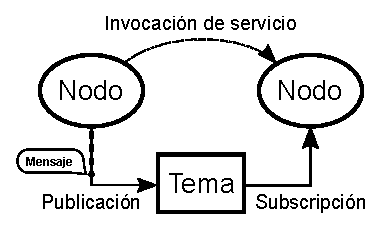
\includegraphics[width=0.5\linewidth]{img/ROS_concepts}
	\caption{Diagrama de comunicación de ROS}
	\label{fig:rosconcepts}
\end{figure}

También están interesantes las animaciones que vienen en la \href{https://docs.ros.org/en/humble/Tutorials/Beginner-CLI-Tools/Understanding-ROS2-Topics/Understanding-ROS2-Topics.html}{página de ROS} \cite{ros2-understanding-topics}, pero lamentablemente no se pueden poner animaciones en el reporte.

\subsection{Nodo (Node)}
\subsection{Tema (Topic)}
\subsection{Mensaje (Message)}
\subsection{Servicio (Service)}
\subsection{Gazebo}
\subsection{RViz}

		
		\section{Dinámica} \label{sec:dinamica}
		\section{Dinámica} \label{sec:dinamica}

La verdad, no les expliqué mucho sobre esta unidad, pero pueden hablar sobre las ecuaciones que vienen en el powerpoint (el cual subí tarde porque se me corrompió)

Hablen sobre el modelo dinámico estandar de un robot, la matriz de masa o inercia, la matriz de coriolis y el vector de gravedad. 

\subsection{Matriz de masa o inercia}
Expliquen cómo el vector de masa o inercia define la aceleración máxima.

\subsection{Matriz de coriolis}

\subsection{Vector de gravedad}

Expliquen por qué el vector de gravedad en su valor máximo (cuando el robot está extendido horizontalmente) debe ser contrarrestado con la fuerza de cada motor

\subsection{Fricción}
Expliquen qué es la fricción en general.

\subsubsection{Fricción estática o seca}

\subsubsection{Fricción dinámica o viscosa}

\subsection{Perturbaciones}
Aquí expliquen qué es una perturbación en general sin profundizar mucho.
	
	% Capítulo 3: Desarrollo
	\chapter{Desarrollo} \label{chap:desarrollo}
	Esta es una pequeña introducción que provee una visión general del Marco Teórico que sustenta el proyecto de robótica. 
Aquí deben definir qué es la \textit{Cinemática}, la \textit{Dinámica} y el uso de \textit{ROS} en robótica. Deben explicar brevemente cómo cada una de estas disciplinas contribuye al control y simulación de manipuladores. Cabe señalar que las ecuaciones principales pueden obtenerse del las diapositivas de PowerPoint o desde los códigos de MATLAB. El apartado de ROS debe completarse con una pequeña búsqueda en Internet para describir su arquitectura básica y casos de uso en simulación.

	
		\section{Características del Robot} \label{sec:caracteristicas_del_robot}
		En esta parte deben de explicar en una tabla 
		
			\subsection{Partes} \label{subsec:partes}
			\subsection{Partes} \label{subsec:partes}
Aquí pondrán la información de las piezas del robot. Pueden eliminar las siguientes subsecciones y simplemente explicar los motores usados y el material de los eslabones porque ya no hay tiempo.
\subsubsection{Motores} \label{subsubsec:motores}
Explicarán cuál es el motor que usaron, harán referencia a la hoja de datos, así como las transmisiones (por ejemplo, las de las pinzas) o reductores de velocidad a los que están acoplados. Deben de poner también información como: masa, fuerza o torque máximo, razón de reducción (por ejemplo, 10/1) y la velocidad máxima.
\subsubsection{Eslabones} \label{subsubsec:eslabones}
Pondrán la masa, inercia, longitud y material de cada eslabón.
			
			\subsubsection{Motores} \label{subsubsec:motores}
			\input{capitulos/Desarrollo/Caracteristicas/Motores}
			
			\subsubsection{Eslabones} \label{subsubsec:eslabones}
			\input{capitulos/Desarrollo/Caracteristicas/Eslabones}
			
			\subsection{Límites y propiedades dinámicas de las articulaciones} \label{subsec:limites_propiedades}
			\subsection{Límites y propiedades dinámicas de las articulaciones} \label{subsec:limites_propiedades}

Básicamente, explicarán lo que aparece en la \autoref{tab:parametros_robot}: Parámetros de Denavit Hartenberg y límites del robot, específicamente lo que aparece después de \code{tipo}. Como no completamos la tarea de dinámica,. pueden comentar esta subsección del documento principal.
		
		\section{Proceso de Cinemática} \label{sec:proceso_cinematica}
		Aquí explicarán su código
Si quieren mostrar un código, pueden hacerlo de la siguiente forma

\begin{minted}{matlab}
	function [q_sol, p_sol] = cinematica_inv(r, p_des, tol, max_iter, alpha, numMuestras)
\end{minted}

Si les sale el error \texttt{latexminted no se reconoce como un comando interno o externo, programa o archivo por lotes ejecutable}, pueden usar 
\begin{terminal}{Instalar minted en python con pip}
	pip install latexminted==0.5.1
\end{terminal}

		
		\section{Control} \label{sec:control}
		\section{Control}
Si quieren, pueden comentar esta parte, pero si quieren, expliquen el diagrama de bloques de la \autoref{fig:diagrama-de-robot-industrial}.

\begin{figure}[h]
	\centering
	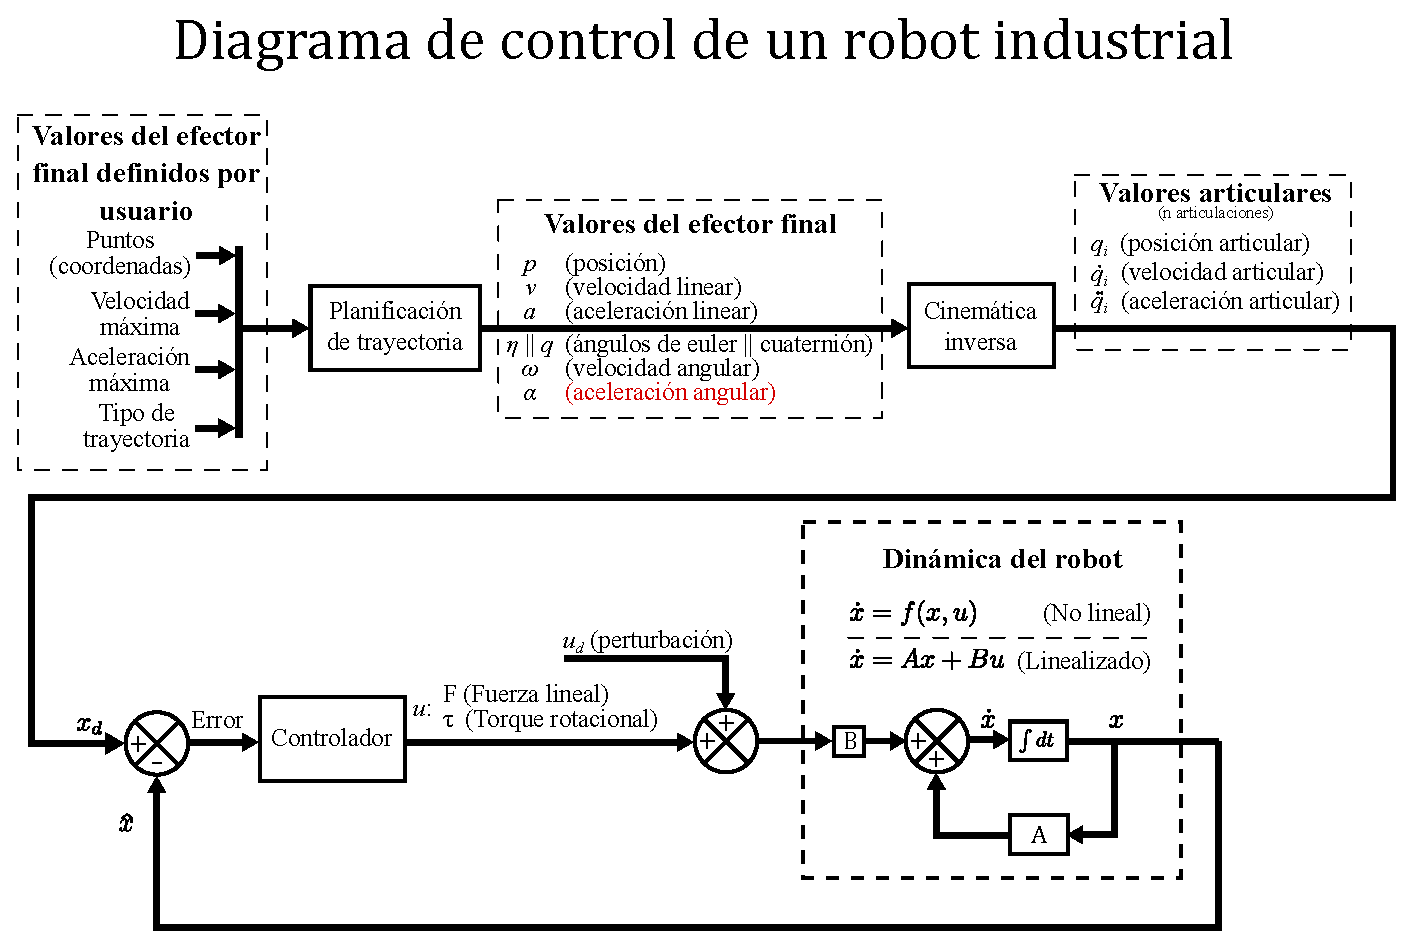
\includegraphics[width=\linewidth]{img/Diagrama_robot_industrial}
	\caption{Diagrama de bloques de un robot industrial}
	\label{fig:diagrama-de-robot-industrial}
\end{figure}

	
	% Capítulo 4: Resultados
	\chapter{Resultados} \label{chap:resultados}
	\chapter{Resultados} \label{chap:resultados}
Aquí pondrán las gráficas que obtuvieron en la simulación de matlab para el robot (si las tienen), y las explicarán.

También mostrarán capturas de pantalla de cómo se ve en Gazebo el robot y en RViz, ya sea que funcione o no, para el cambio de trayectoria. Describirán lo que ocurre y por qué (si es que saben).

	
	% Capítulo 5: Conclusiones
	\section{Conclusiones} \label{sec:conclusiones}
	\section{Juancito}
Conclusiones y comentarios de Juancito, explicando los problemas que tuvo y lo que aprendió.
	\section{Panchito}
Conclusiones y comentarios de Panchito, explicando los problemas que tuvo y lo que aprendió.
	\section{Lupita}
Conclusiones y comentarios de Lupita, explicando los problemas que tuvo y lo que aprendió.
	\section{Pepito}
Conclusiones y comentarios de Pepito, explicando los problemas que tuvo y lo que aprendió.
		
	
	\titleformat{\chapter}
	{\bfseries\huge}
	{}
	{0pt}
	{~\raisebox{-1.5pt}{}
		\\\vspace{.05cm}\titlerule\\\filcenter #1 \\\vspace{.25cm}\titlerule}
	%{\titlerule\\\vspace{.25cm}\filcenter #1 \\\vspace{.25cm}\titlerule}
	\bibliographystyle{IEEEtranN}
	\newpage\label{bibliografia}
	\addcontentsline{toc}{chapter}{Bibliografía}\bibliography{bibliografia}
\end{document}


